\documentclass[../../dd.tex]{subfiles}

% Document
\begin{document}
    \chapter{Architectural Design}
    \section{Overview}
    From an external point of view, users using their smartphones exploit the different
    services offered by \textit{Baddy} that are different for clients and caregivers.
    The application to be developed is based on one application component (application logic) which manages the interactions
    between different components of the system.
    Application logic is present both in the mobile view and in the back-end logic.
    In the mobile view there is the management of the GUI and the connection with other useful components
    present in the smartphone like GPS and camera; in the back-end logic instead there is the most of the logic and also the interfaces to external services:
    Database provider, Storage provider and Push notification provider.


    \begin{figure}[H]
        \centering
        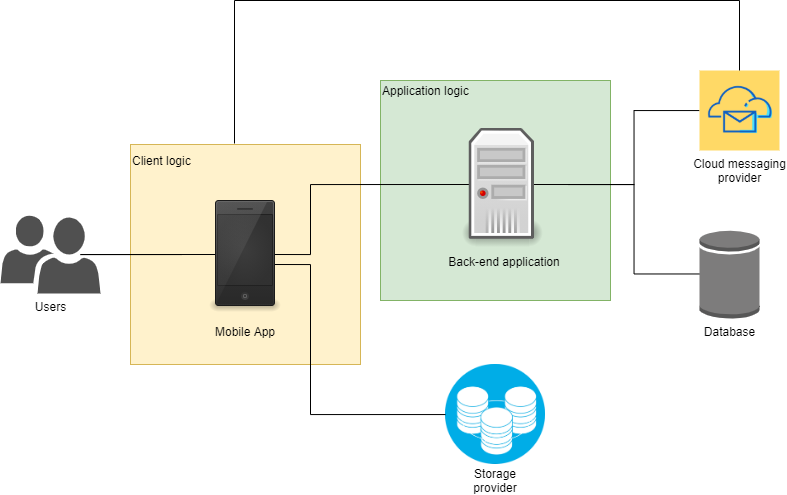
\includegraphics[scale=0.5]{assets/overview.png}\\[1.6 cm]
        \caption[\textit{Deployment} Diagram]{Overview of the application components}
    \end{figure}
    %todo add photo
    \section{Component View}
    %todo add photo
    In this section the system will be described in terms of its components: their
    functionalities will be discussed and detailed. Moreover, interfaces among components and among external systems will be shown.\\

    \begin{figure}[H]
        \centering
        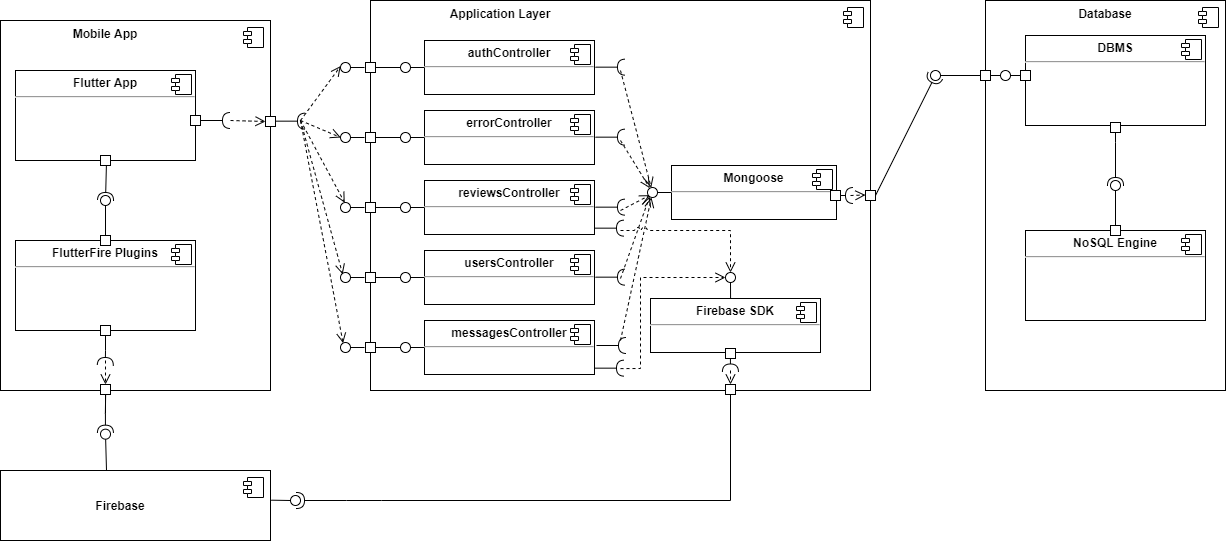
\includegraphics[scale=0.35]{assets/component.png}\\[1.6 cm]
        \caption[Component diagram]{Component diagram}
    \end{figure}

    \subsection{Database}
    The application database is managed using a Non-Relational DBMS.
    It allows the reading of data, ensuring to the users the possibility to log in and check the stored data.
    It is also used for data manipulation (insertion, modification and deletion).
    The database offers to the Application Server an interface that it can use
    to interact with it.
    Particular attention must be paid to the encryption of passwords used to the user access to the system.

    \subsection{Application Server}
    The main feature of the Application Server is to define rules and work-flows
    of all the functionalities defined by the RestfulAPI.
    The Application Server must have interfaces to communicate with the Mobile
    Application and also with the DBMS; the communication must be done using
    the HTTPS protocol.
    In the brief introduction below, logic modules and their descriptions are
    presented, while all the connections among them can be seen in the Global
    Component View.
    \begin{itemize}
        \item \textbf{authController:} This module handles the authentication and authorization process.
        It generates authorization tokens and checks their validity.
        \item \textbf{errorController:} It manages all the routes that are not available and all the bad formatted requests.
        \item \textbf{handlerFactory:} General service that implements all CRUD operations.
        \item \textbf{reviewsController:} It manages all the newly created reviews with all the rankings.
        \item \textbf{usersController:} It manages users operations, like insertion of a new offer and updating
        profile.
        \item \textbf{messagesController:} It manages all the messages sent by clients to caregivers' profiles
    \end{itemize}

    \subsection{Mobile Application}
    The mobile application communicates with the Application Server
    through RestfulAPIs that are defined in order to describe the interactions
    between the two layers and that must be independent of the two implementations. More details about the implementation will be provided in the following sections.

    \newpage
    \section{Deployment View}
    In this section a deployment diagram details the execution architecture of the system, including nodes such as hardware or software execution environments, and the middleware connecting them.

    \begin{figure}[H]
        \centering
        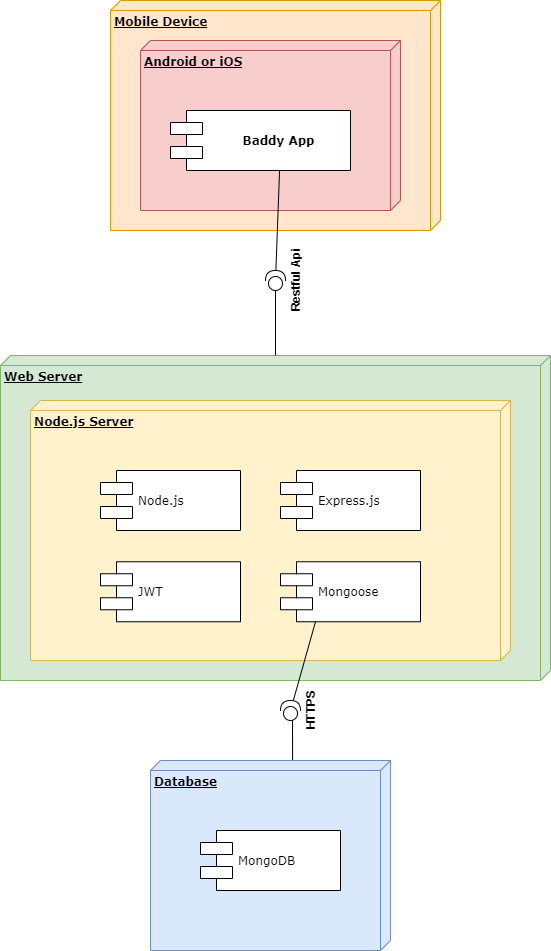
\includegraphics[scale=0.5]{assets/deployment2.png}\\[1.6 cm]
        \caption[\textit{Deployment} Diagram]{ Deployment diagram}
    \end{figure}


    \section{Selected architectural styles and Patterns}
    This section details the architectural styles and patterns used to design the system architecture. In the following sections, the different patterns will be explained in terms of styles, principles and why we chose them.

    \subsection{State Management with Provider} Managing State using setState() starts becoming heavy as the code grows, because whenever you need to change the widget’s UI, you have to call setState() inside the changing widget, so that it gets rebuilt, and since application is composed of hundreds of different widgets, there could be hundred different points where you have to take care of calling setState(), and managing state. Thus, using this raw technique to manage state is not a good option, but thankfully we have a better approach, which is not just easy but effective, called Provider State Management. Moreover, thanks to provider, we can access the model easily with a single line of code, without the need of passing the instance down to the tree of the widgets that would make the code difficult to understand and maintain.


    \subsection{Representational state transfer} REST is a software architectural style that
    defines a set of constraints to be used for creating Web services. RESTful
    Web services allow the requesting systems to access and manipulate textual
    representations of Web resources by using a uniform and predefined set of
    stateless operations.
    In order for an API to be considered RESTful, it has to conform to these main criteria:
    \begin{itemize}
        \item A client-server architecture made up of with requests managed through HTTP.
        \item Stateless client-server communication, i.e. each request is separate and unconnected.
        \item A uniform interface between components so that information is transferred in a standard form.
    \end{itemize}
    Resources are decoupled from their representation so that their content can be accessed in a variety of formats, such as HTML, XML, plain text, PDF, JPEG, JSON, and others. This improves the independence of the various tiers of the system. This pattern is used to develop APIs for communications between the application server with the mobile client and the application server.


    \subsection{Multi-tier architecture} In the Multi-tier Architecture pattern, the components
    of the system are placed on different physical layers, which are not
    isolated, but they communicate through interfaces with at least another layer
    of the system. The main benefits of a multi-tier architecture are:
    \begin{itemize}
        \item  different tiers of an application gives development teams the
        ability to develop and enhance a product with higher speed than developing
        a unique code base because a specific layer can be upgraded with minimal
        impact on the other layers;
        \item scalability is another great benefit of a multi-tier
        architecture. By distributing the different layers you can scale each
        autonomously depending on the need at any given time;
        \item  having different layers can also increase the system’s reliability and availability
        by hosting different parts of your application on different servers.
    \end{itemize}

    \subsection{Thin client} A thin client is a lightweight component that has been optimized for establishing a remote connection with a server-based computing environment.
    A thin client is an advantage because all the application logic is allocated on the application server, which has enough computational power to manage concurrency efficiently.

    \subsection{Other design decisions}
    \subsection{Security}
    All the information regarding users are sensitive. The system must prevent any attack that could steal data or make the service unavailable. The data exchanged will be encrypted by the mean of the HTTPs protocol that relies on SSL/TLS. The system will never expose any sensible data with external actors without the user's consent.



\end{document}
